\section{Thông tin nhóm}
-   Tên học phần: Mạng máy tính. \\
-   Đồ án thực hiện: Lập trình Socket. \\
-   Thời gian thực hiện: 23/11/2025 đến ngày 14/12/2025. \\
-   Danh sách thành viên: \\
\begin{table}[h!]
\centering
\begin{tabular}{|c|c|l|l|}
\hline
\textbf{STT} & \textbf{MSSV} & \textbf{Họ và tên} & \textbf{Vai trò} \\ \hline
01           & 23127004      & Nguyễn Khánh Linh        & Thành viên      \\ \hline
02           & 23127113      & Trần Hoàng Phúc & Nhóm trưởng    \\ \hline
03           & 23127165      & Nguyễn Hữu Gia Minh     & Thành viên      \\ \hline
\end{tabular}
\end{table}

\section{Thông tin đồ án}

\subsection{Tổng quan đồ án}
\begin{itemize}
    \item \textbf{Yêu cầu:} Xây dựng một hệ thống trình phát video trực tuyến gồm client và server, sử dụng:
    \begin{itemize}
        \item \textbf{RTSP (Real-Time Streaming Protocol):} Giao thức điều khiển trên TCP
        \item \textbf{RTP (Real-time Transport Protocol):} Giao thức truyền dữ liệu media trên UDP
    \end{itemize}
    \item \textbf{Mục đích:} Hiểu rõ về các giao thức mạng thời gian thực, quản lý trạng thái phiên kết nối, và kỹ thuật đóng gói (packetization) dữ liệu đa phương tiện.
\end{itemize}

\subsection{Mục tiêu}
\begin{itemize}
    \item Triển khai giao thức RTSP phía client để gửi các lệnh điều khiển (SETUP, PLAY, PAUSE, TEARDOWN).
    \item Triển khai RTP packetization phía server để gửi video dạng MJPEG tới client.
    \item Hiểu và quản lý trạng thái phiên RTSP.
    \item Hỗ trợ HD Video Streaming và Client-Side Caching để cải thiện chất lượng phát video.
\end{itemize}

\subsection{Kiến trúc hệ thống}

\subsubsection{Kênh điều khiển (RTSP)}
\begin{itemize}
    \item Sử dụng TCP để truyền các lệnh RTSP.
    \item Port mặc định: 554 (TCP).
    \item Client gửi các lệnh:
    \begin{itemize}
        \item \textbf{SETUP:} Thiết lập phiên kết nối và thông số transport.
        \item \textbf{PLAY:} Bắt đầu phát video.
        \item \textbf{PAUSE:} Tạm dừng phát video.
        \item \textbf{TEARDOWN:} Kết thúc phiên kết nối.
    \end{itemize}
    \item Mỗi lệnh RTSP phải kèm CSeq header (số thứ tự lệnh) và Session header (mã phiên) nếu cần.
\end{itemize}

\subsubsection{Kênh dữ liệu (RTP)}
\begin{itemize}
    \item Sử dụng UDP để truyền dữ liệu video.
    \item Server thực hiện RTP packetization:
    \begin{itemize}
        \item Header gồm các trường: V, P, X, CC, M, PT, Sequence Number, Timestamp, SSRC.
        \item Payload là dữ liệu video MJPEG.
    \end{itemize}
    \item Client nhận RTP packet và giải mã để hiển thị video.
\end{itemize}

\subsubsection{Client}
\begin{itemize}
    \item Client cần triển khai hành vi khi người dùng nhấn các nút điều khiển:
    \begin{itemize}
        \item Mở kết nối RTSP với server khi khởi động.
        \item Gửi và nhận các lệnh RTSP.
        \item Quản lý trạng thái phiên (INIT, READY, PLAYING).
        \item Nhận và hiển thị dữ liệu RTP.
    \end{itemize}
\end{itemize}

\subsubsection{Server}
\begin{itemize}
    \item Server đọc video MJPEG từ file và gửi từng frame dưới dạng RTP packet.
    \item Server phản hồi tất cả các lệnh RTSP từ client (200 OK, 404 FILE\_NOT\_FOUND, 500 CONNECTION\_ERROR).
    \item RTP packetization:
    \begin{itemize}
        \item V = 2, P = X = CC = M = 0, PT = 26 (MJPEG), Sequence Number theo frame, Timestamp từ Python time module, SSRC tự chọn.
    \end{itemize}
\end{itemize}

\subsection{Yêu cầu kỹ thuật}

\subsubsection{PHẦN 1: Triển khai Client}

\paragraph{A. Các Module}
\begin{itemize}
    \item \textbf{ClientLauncher:} Khởi động giao diện người dùng (không cần sửa)
    \item \textbf{Client:} Xử lý logic RTSP (cần hoàn thiện)
\end{itemize}

\paragraph{B. Triển Khai RTSP Commands}

\paragraph{1. Lệnh SETUP}
\begin{itemize}
    \item \textbf{Mục đích:} Thiết lập phiên làm việc và tham số truyền tải
    \item \textbf{Công việc cần làm:}
    \begin{itemize}
        \item Tạo UDP socket để nhận dữ liệu RTP từ Server
        \item Thiết lập timeout = 0.5 giây cho socket
        \item Gửi RTSP request đến Server:
        \begin{itemize}
            \item CSeq: Số thứ tự lệnh (bắt đầu từ 1)
            \item Transport: RTP/UDP; client\_port=<RTP\_port>
        \end{itemize}
        \item Nhận response từ server
        \item Parse Session ID từ header response để sử dụng cho các lệnh sau
    \end{itemize}
\end{itemize}

\paragraph{2. Lệnh PLAY}
\begin{itemize}
    \item \textbf{Mục đích:} Bắt đầu phát video
    \item \textbf{Công việc cần làm:}
    \begin{itemize}
        \item Gửi request PLAY với headers:
        \begin{itemize}
            \item CSeq: Tăng lên 1 so với lệnh trước
            \item Session: Session ID nhận được từ SETUP
            \item KHÔNG có Transport header
        \end{itemize}
        \item Nhận và xử lý response từ server
        \item Cập nhật trạng thái client sang PLAYING
    \end{itemize}
\end{itemize}

\paragraph{3. Lệnh PAUSE}
\begin{itemize}
    \item \textbf{Mục đích:} Tạm dừng phát video
    \item \textbf{Công việc cần làm:}
    \begin{itemize}
        \item Gửi request PAUSE với headers:
        \begin{itemize}
            \item CSeq: Tăng lên 1
            \item Session: Session ID
            \item KHÔNG có Transport header
        \end{itemize}
        \item Nhận response
        \item Cập nhật trạng thái client sang READY
    \end{itemize}
\end{itemize}

\paragraph{4. Lệnh TEARDOWN}
\begin{itemize}
    \item \textbf{Mục đích:} Kết thúc phiên và đóng kết nối
    \item \textbf{Công việc cần làm:}
    \begin{itemize}
        \item Gửi request TEARDOWN với headers:
        \begin{itemize}
            \item CSeq: Tăng lên 1
            \item Session: Session ID
            \item KHÔNG có Transport header
        \end{itemize}
        \item Nhận response
        \item Đóng socket và cập nhật trạng thái về INIT
    \end{itemize}
\end{itemize}

\textbf{C. Định Dạng RTSP Message}

\begin{itemize}
    \item \textbf{Request Format:}
    \begin{verbatim}
<METHOD> <video_file> RTSP/1.0
CSeq: <sequence_number>
[Session: <session_id>]
[Transport: RTP/UDP; client_port=<port>]
    \end{verbatim}
    
    \item \textbf{Response Format:}
    \begin{verbatim}
RTSP/1.0 <status_code> <status_message>
CSeq: <sequence_number>
Session: <session_id>
    \end{verbatim}
    
    \item \textbf{Mã trạng thái:}
    \begin{itemize}
        \item 200: Thành công
        \item 404: File không tìm thấy
        \item 500: Lỗi kết nối
    \end{itemize}
\end{itemize}

\begin{figure}[H]
\centering
\begin{tikzpicture}[
    state/.style={rectangle, draw, minimum width=2cm, minimum height=1cm, align=center},
    arrow/.style={->, thick}
]
    \node[state] (init1) {INIT};
    \node[state, below=2cm of init1] (ready) {READY};
    \node[state, below=2cm of ready] (playing) {PLAYING};
    \node[state, below=2cm of playing] (init2) {INIT};
    
    \draw[arrow] (init1) -- node[right] {SETUP} (ready);
    \draw[arrow] (ready) -- node[right] {PLAY} (playing);
    \draw[arrow] (playing) to[bend left=45] node[left] {PAUSE} (ready);
    \draw[arrow] (ready) to[bend left=45] node[right] {} (playing);
    \draw[arrow] (playing) -- node[right] {TEARDOWN} (init2);
\end{tikzpicture}
\caption{RTSP State Machine}
\end{figure}

\begin{figure}[H]
    \centering
    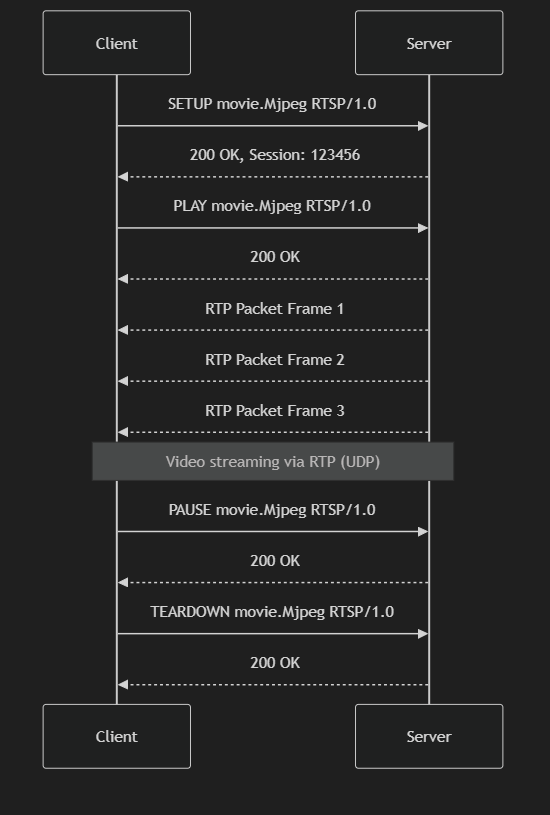
\includegraphics[width=0.8\textwidth]{DIAGRAM1.png}
    \caption{Sơ đồ kiến trúc hệ thống}
\end{figure}

\clearpage
